%%%%%%%%%%%%%%%%%%%%%%%%%%%%%%%%%%%%%%%%%
% Beamer Presentation
% LaTeX Template
% Version 1.0 (10/11/12)
%
% This template has been downloaded from:
% http://www.LaTeXTemplates.com
%
% License:
% CC BY-NC-SA 3.0 (http://creativecommons.org/licenses/by-nc-sa/3.0/)
%
%%%%%%%%%%%%%%%%%%%%%%%%%%%%%%%%%%%%%%%%%

%----------------------------------------------------------------------------------------
%	PACKAGES AND THEMES
%----------------------------------------------------------------------------------------

\documentclass{beamer}

\mode<presentation> {

% The Beamer class comes with a number of default slide themes
% which change the colors and layouts of slides. Below this is a list
% of all the themes, uncomment each in turn to see what they look like.

%\usetheme{default}
%\usetheme{AnnArbor}
%\usetheme{Antibes}
%\usetheme{Bergen}
%\usetheme{Berkeley}
%\usetheme{Berlin}
%\usetheme{Boadilla}
%\usetheme{CambridgeUS}
%\usetheme{Copenhagen}
%\usetheme{Darmstadt}
%\usetheme{Dresden}
%\usetheme{Frankfurt}
%\usetheme{Goettingen}
%\usetheme{Hannover}
%\usetheme{Ilmenau}
%\usetheme{JuanLesPins}
%\usetheme{Luebeck}
\usetheme{Madrid}
%\usetheme{Malmoe}
%\usetheme{Marburg}
%\usetheme{Montpellier}
%\usetheme{PaloAlto}
%\usetheme{Pittsburgh}
%\usetheme{Rochester}
%\usetheme{Singapore}
%\usetheme{Szeged}
%\usetheme{Warsaw}

% As well as themes, the Beamer class has a number of color themes
% for any slide theme. Uncomment each of these in turn to see how it
% changes the colors of your current slide theme.

%\usecolortheme{albatross}
%\usecolortheme{beaver}
%\usecolortheme{beetle}
%\usecolortheme{crane}
%\usecolortheme{dolphin}
%\usecolortheme{dove}
%\usecolortheme{fly}
%\usecolortheme{lily}
%\usecolortheme{orchid}
%\usecolortheme{rose}
%\usecolortheme{seagull}
%\usecolortheme{seahorse}
%\usecolortheme{whale}
%\usecolortheme{wolverine}

%\setbeamertemplate{footline} % To remove the footer line in all slides uncomment this line
%\setbeamertemplate{footline}[page number] % To replace the footer line in all slides with a simple slide count uncomment this line

%\setbeamertemplate{navigation symbols}{} % To remove the navigation symbols from the bottom of all slides uncomment this line
}

\usepackage{graphicx} % Allows including images
\usepackage{booktabs} % Allows the use of \toprule, \midrule and \bottomrule in tables

%----------------------------------------------------------------------------------------
%	TITLE PAGE
%----------------------------------------------------------------------------------------

\title[AI and the Supreme Court]{What AI can tell us about the U.S. Supreme Court} % The short title appears at the bottom of every slide, the full title is only on the title page

\author{Eric Chuu} % Your name
\institute[UCLA] % Your institution as it will appear on the bottom of every slide, may be shorthand to save space
{
University of California, Los Angeles \\ % Your institution for the title page
%\medskip
%\textit{@smith.com} % Your email address
}
\date{\today} % Date, can be changed to a custom date

\begin{document}

\begin{frame}
\titlepage % Print the title page as the first slide
\end{frame}

\begin{frame}
\frametitle{Overview} % Table of contents slide, comment this block out to remove it
\tableofcontents % Throughout your presentation, if you choose to use \section{} and \subsection{} commands, these will automatically be printed on this slide as an overview of your presentation
\end{frame}

%----------------------------------------------------------------------------------------
%	PRESENTATION SLIDES
%----------------------------------------------------------------------------------------

%------------------------------------------------
\section{Background of the article}

\section{Model Details} % Sections can be created in order to organize your presentation into discrete blocks, all sections and subsections are automatically printed in the table of contents as an overview of the talk
%------------------------------------------------

\section{AI, Machine Learning in the Model}
\subsection{Text-Based Analysis}
\subsection{Cross Validation}
%\subsection{How does machine learning help predict a process that occurs behind closed doors} % A subsection can be created just before a set of slides with a common theme to further break down your presentation into chunks
%\subsection{Details of the methods used in this particular model}

\section{Future Considerations}
\subsection{Extended models}

\section{Conclusion}


\begin{frame}
\frametitle{Background}
\begin{itemize}
	 \item Lifetime tenure of the U.S. Supreme Court's justices
	 \item People have vested interest in their decisions and deliberations
	 \item Model the Supreme Court's decision-making process
	 \item Identify which of the nine justices were likely to ``swing," or waver on certain issues
\end{itemize}

\begin{figure}[h]
\begin{center}
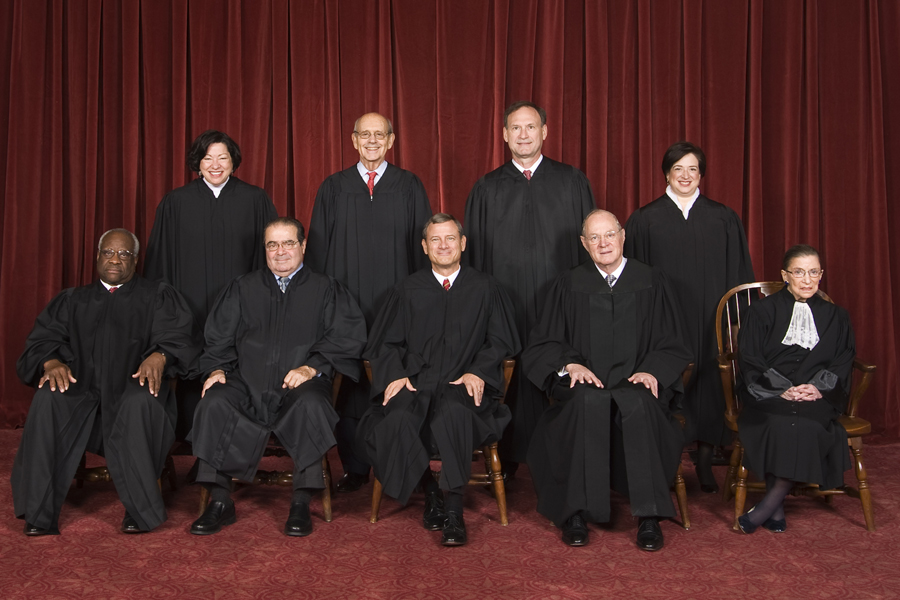
\includegraphics[width=0.6\columnwidth]{roberts6}
\end{center}
\end{figure}


\end{frame}

%------------------------------------------------

\begin{frame}
\frametitle{Background}
\begin{itemize}
\item Process of deliberation
	\begin{itemize}
		\item Initial stance
		\item Hearing
		\item Decision made during private meeting
		\item Write opinions % talk about difficulty of interpreting opinions because they can be written by more than one justice, and they express conflicting opinions
	\end{itemize}
\item Old models pinpointed news converage, voting records as predictors for a justice's stance on a particular issue
\item Supreme Court Ideal Pointer Minter (SCIPM): incorporates text analysis
\end{itemize}
\end{frame}

%------------------------------------------------

\begin{frame}
\frametitle{Model Details}

\begin{itemize}
	\item Cases often have many different issues
	\item Model looked at opinion text that the justice writes
	\item Correlation between the text and how each justice feels on particular issue
	\item Model generated a spectrum of specific issues justices' views % swing justices in the middle -- the most moderate ones, put the picture of the visual into the slide
\end{itemize}

\end{frame}

%------------------------------------------------
\begin{frame}
\frametitle{Model Details}


\begin{figure}[h]
\begin{center}
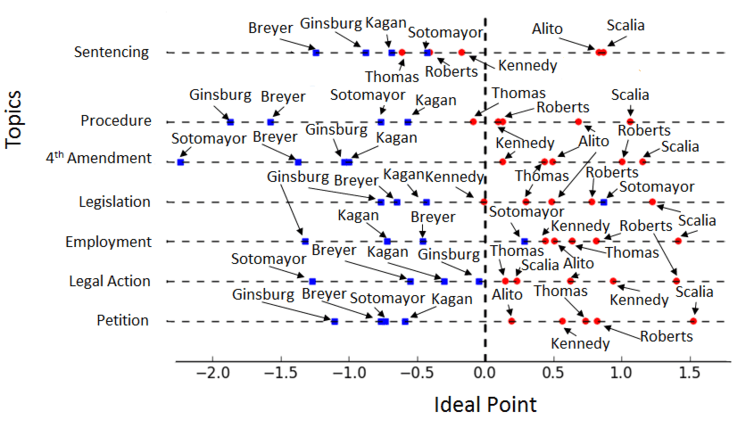
\includegraphics[width=1.0\columnwidth]{model_visual}
\end{center}
\end{figure}


\end{frame}

%------------------------------------------------


\begin{frame}
\frametitle{Model Details}
\begin{columns}[c] % The "c" option specifies centered vertical alignment while the "t" option is used for top vertical alignment

\column{.45\textwidth} % Left column and width
\textbf{Checking the Model}
\begin{enumerate}
\item Looked at cases that were decided by a 5-4 margin
\item Identify the swing justices
\item Kennedy, Roberts, Thomas were often in the same group, consistent with the model's predictions
\end{enumerate}

\column{.5\textwidth} % Right column and width
Other observations: Top voter was Kennedy, decisions tended to cluster based on political party

\end{columns}
\end{frame}

%------------------------------------------------
%\section{Second Section}
%------------------------------------------------

\begin{frame}
\frametitle{AI/Machine Learning in the Model}
\textbf{Text-Based Analysis}
\begin{enumerate}
	\item Two types: topic analysis and sentiment analysis
	\item Model combined the two to use historical opinion text to ``learn" and classify the decisions when reading new opinion text
	\item The model looked at: number of words, identifies key words that pertain to each issue, assigns a weight to each issue
	\item Classification problem
\end{enumerate}


\begin{figure}[h]
\begin{center}
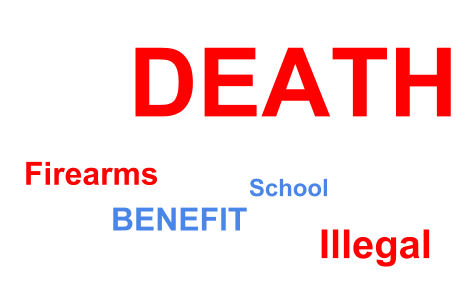
\includegraphics[width=0.65\columnwidth]{text}
\end{center}
\end{figure}



\end{frame}



%-----------------------------------------

\begin{frame}
\frametitle{Classification Example}
\textbf{Before Classification}

\begin{figure}[h]
\begin{center}
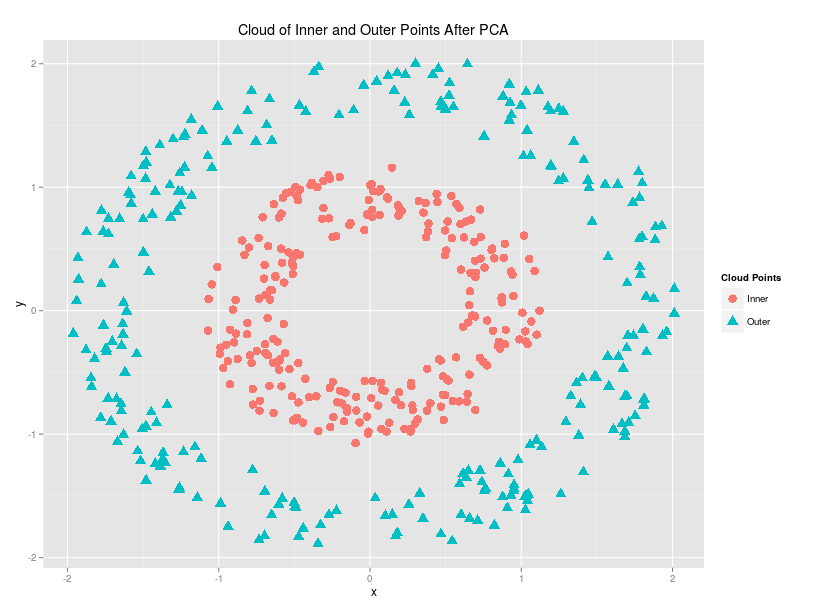
\includegraphics[width=0.75\columnwidth]{pre_class}
\end{center}
\end{figure}

\end{frame}

%------------------------------------------

\begin{frame}
\frametitle{Classification Example}
\textbf{After Classification}
\begin{figure}[h]
\begin{center}
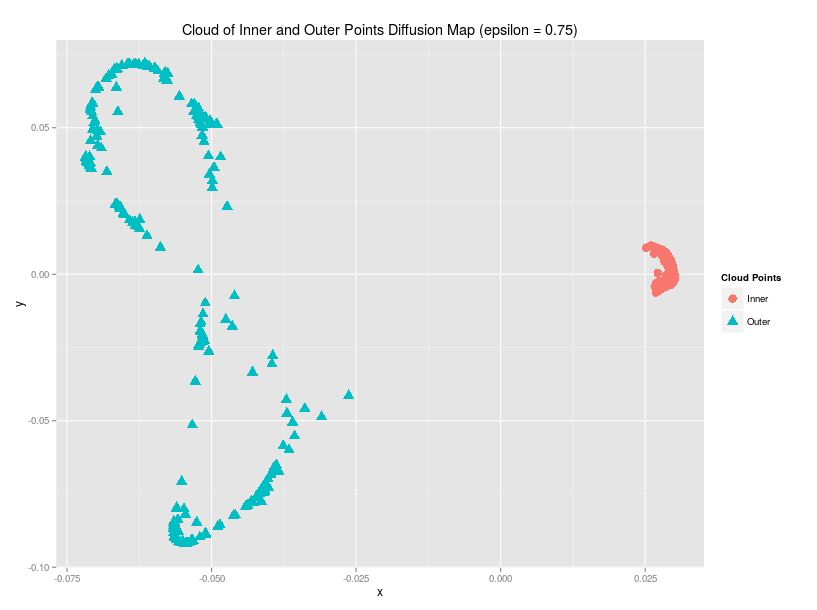
\includegraphics[width=0.75\columnwidth]{post}
\end{center}
\end{figure}

\end{frame}


%------------------------------------------------

\begin{frame}
\frametitle{Cross Validation}
%\begin{theorem}[Mass--energy equivalence]
%$E = mc^2$
%\end{theorem}

\begin{definition} [Cross Validation]
A model validation technique for assessing how the results of a statistical analysis will generalize to an independent data set.
\end{definition}

\begin{itemize}
	\item Training set vs. Test (Validation) set
	\item K-Fold Cross Validation
\end{itemize}

\begin{figure}[h]
\begin{center}
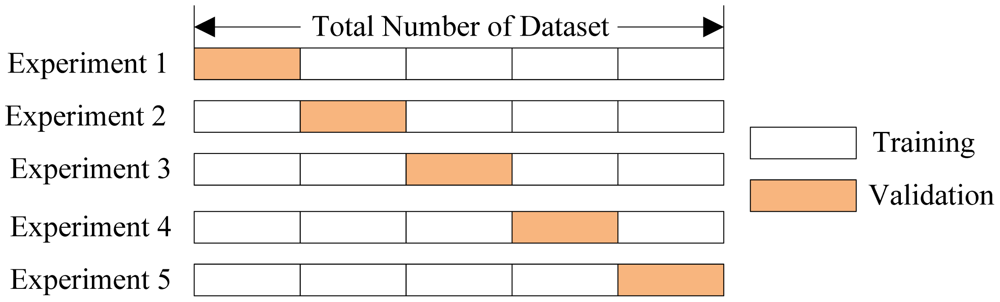
\includegraphics[width=0.9\columnwidth]{kfold}
\end{center}
\end{figure}




\end{frame}



%------------------------------------------------

\begin{frame}[fragile] % Need to use the fragile option when verbatim is used in the slide
\frametitle{Future Considerations}
\textbf{Additions to the Current Model}
\begin{itemize}
	\item Evaluate public response: social media, popular cases
	\item Use text transcripts of oral discussion
	\item Natural Language Processing (NLP)
	\begin{itemize}
		\item Using computers to find meaning in human language
	\end{itemize}
\end{itemize}


\end{frame}

%------------------------------------------------
\begin{frame}
\frametitle{Conclusion}

\begin{itemize}
	\item Text-based analysis becoming more flexible in application: election outcomes, customer feedback, etc.
\end{itemize}

\begin{figure}[h]
\begin{center}
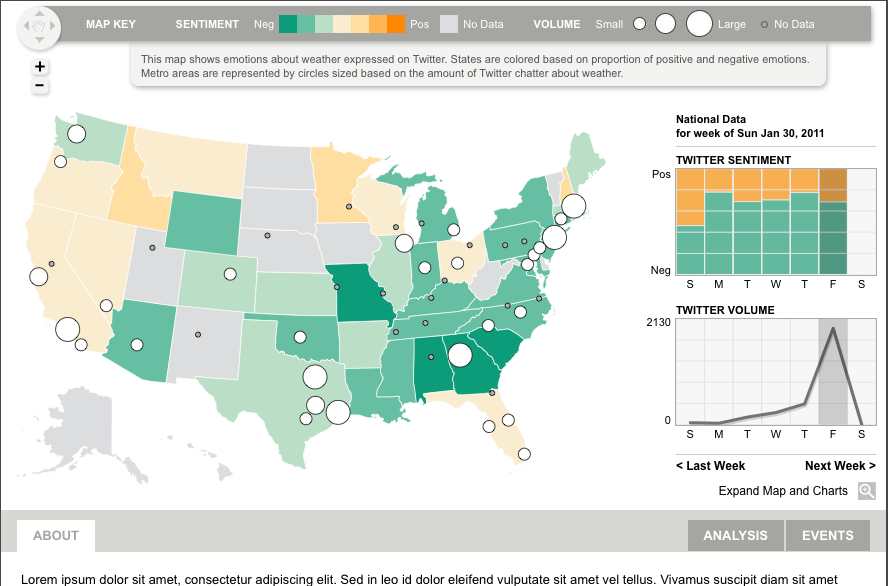
\includegraphics[width=0.8\columnwidth]{weather}
\end{center}
\end{figure}
\end{frame}

	
\begin{frame}
\frametitle{Conclusion}

\begin{itemize}	
	\item Machine Learning/AI advancements and improving techniques leading to increased insight into previously hidden processes
	\item The model, if improved, can gauge in which direction the judicial system is headed: political, social, economic stances of the justices
		\begin{itemize}
			\item Alter perception of judicial system and incite potential changes
		\end{itemize}
\end{itemize}


\end{frame}



%------------------------------------------------

\begin{frame}
\frametitle{Bibliography}
\footnotesize{
\begin{thebibliography}{9}

\bibitem{Fang} J. Fang, \emph{How Text Analytics Works},  Medallia

\bibitem{supcourt}
M. R. Islam, T. Hossain, S. Krishnan \emph{What AI can tell us about the U.S. Supreme Court}, The Conversation, 2016.

\bibitem{lee} B. Pang, L. Lee, \emph{Opinion mining and sentiment analysis}, now the essence of knowledge, 2008

\bibitem{weather} T. Masterman, \emph{Hope for Human Sentiment Analysis Coding},  Dialogue Earth, May 13, 2011



\end{thebibliography}

}
\end{frame}

%------------------------------------------------

%----------------------------------------------------------------------------------------

\end{document} 